\documentclass[mathserif]{beamer}
\usepackage{amsmath}
\mode<presentation>
\usetheme{Madrid}
\AtBeginSection[]{}
\title{Phase Transitions and Scale Free Phenomena in Networks of Memristive Elements}
\author{Forrest Sheldon}
\institute{UCSD}
\date{August 7, 2015}
\titlegraphic{
\includegraphics[width=2.5cm]{gl-1-logo.png}}
\begin{document}

\begin{frame}
\titlepage
\end{frame}

\begin{frame}
\frametitle{A Perspective On Memristors}

\begin{columns}
\column{0.5\textwidth}
\centering
\onslide<1->{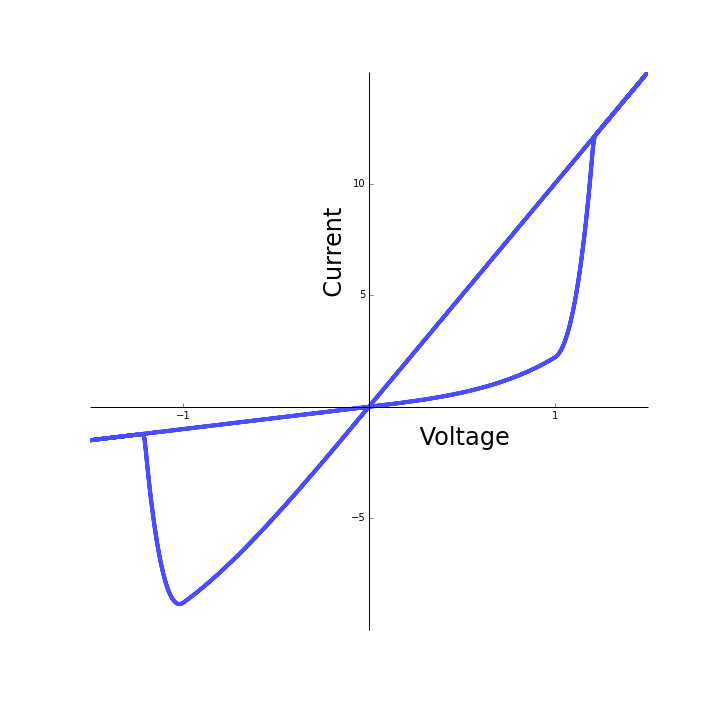
\includegraphics[width=0.8\textwidth]{hysteresis.png}}
\column{0.5\textwidth}
\centering
\onslide<3->{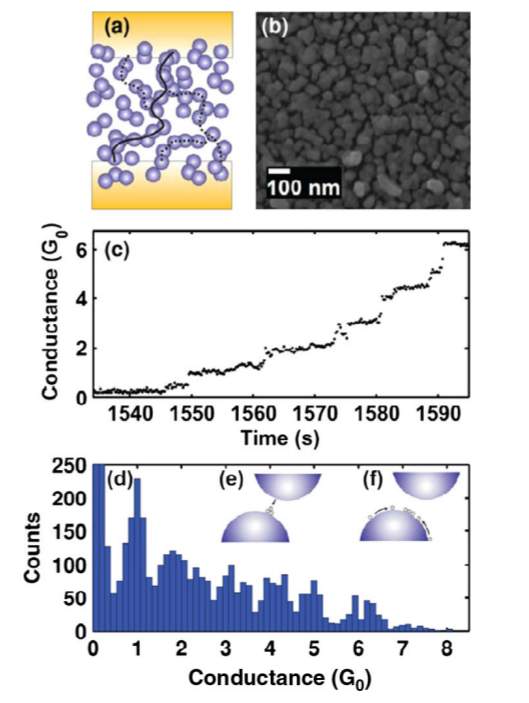
\includegraphics[width=0.6\textwidth]{Granular_Material.png}}
\end{columns}
\begin{center}
\onslide<2->{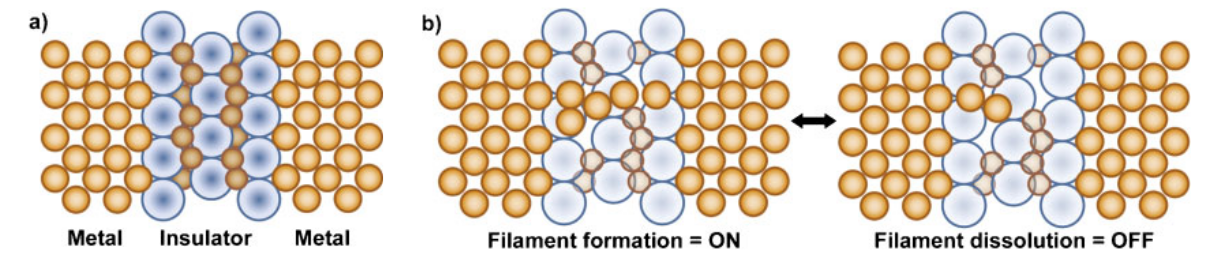
\includegraphics[width=\textwidth]{Atomic_Switch_Filament.png}}
\end{center}
\end{frame}

\begin{frame}
\frametitle{'Nonideal' Properties are interesting}

\begin{center}
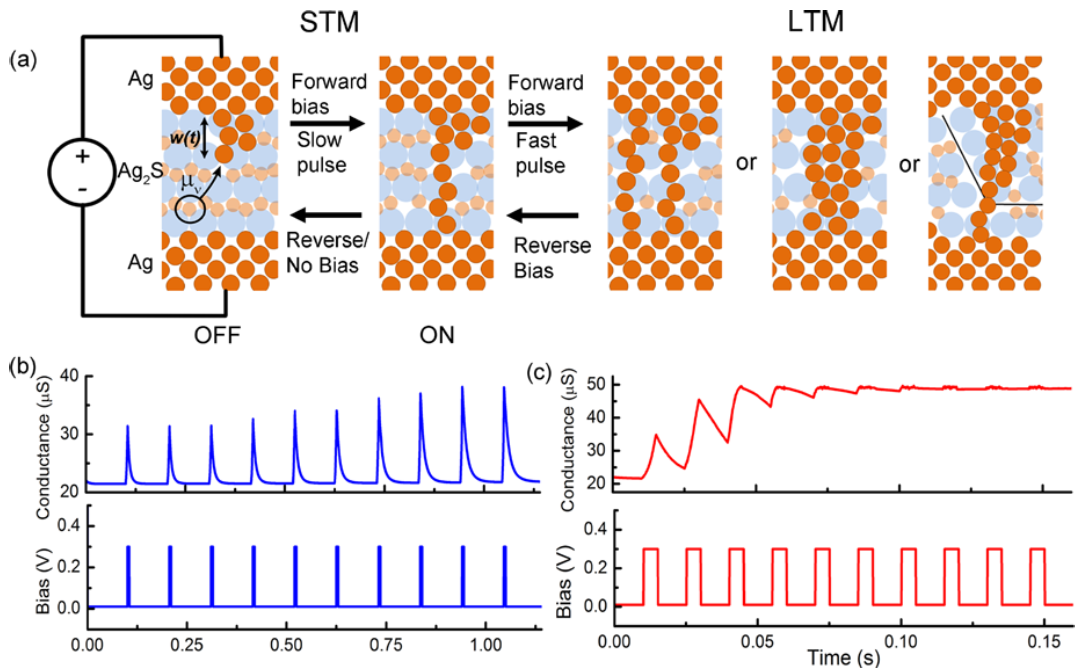
\includegraphics[width=0.8\textwidth]{STM_LTP.png}
\end{center}

\end{frame}

\begin{frame}
\frametitle{Atomic Switch Networks}

\begin{center}
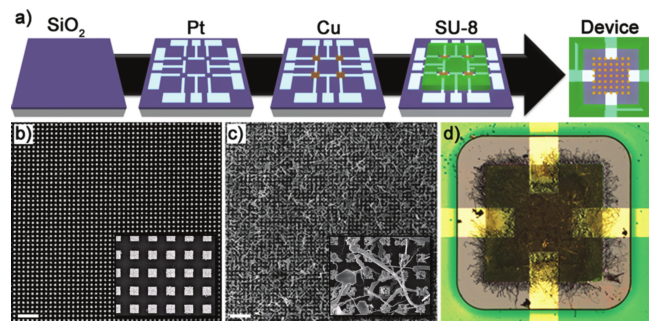
\includegraphics[width=9cm]{ASN_fabrication.png}
\end{center}

\end{frame}

\begin{frame}
\frametitle{Questions}
\begin{itemize}
\item How can we see the memristive cycling, which is a collective action of the network,
in the language of phase transitions?
\item How do the parameters of the devices affect the presence of a transition?
\item The full time integration is too difficult to discern a transition or avalanches.
What features can we discard?
\item Can these networks display SOC or scaling about these transitions?
\end{itemize}
\end{frame}

\begin{frame}
\frametitle{Memristor Network Model}
\begin{itemize}
\item Memristive switching is fast compared to external control
but slow compared to electrons $\to$ at any time point, networks are
ohmic but individual memristors switch discontinuously between
$g_{OFF}$ and $g_{ON}$
\item Thresholds are essential to causal structure of switching
\item Most behaviors are robust to network structure $\to$ pick any canonical disordered network
\item Disorder induces a voltage distribution over the network $\to$ absorb voltage disorder into
thresholds and simulate on regular lattice with disordered thresholds
\item Memristors act like switches that transition from a thermodynamically favored OFF state
to ON when the current passes some random threshold $t_i$ drawn from a distribution $p(t)$
\item Possible Caveats
\end{itemize}

\end{frame}

\begin{frame}
\frametitle{Simulation Results}
\begin{itemize}
\item $g_{ON} / g_{OFF} = 2$
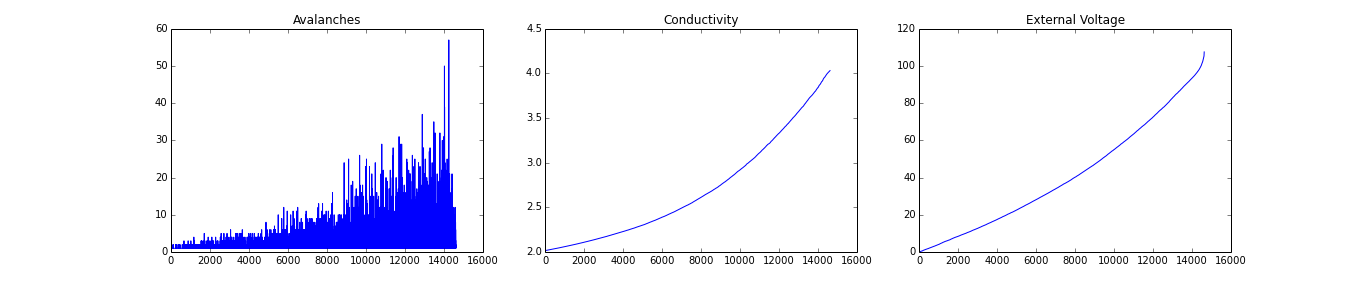
\includegraphics[width=0.8\textwidth]{ON2_run.png}
\item $g_{ON} / g_{OFF} = 100$
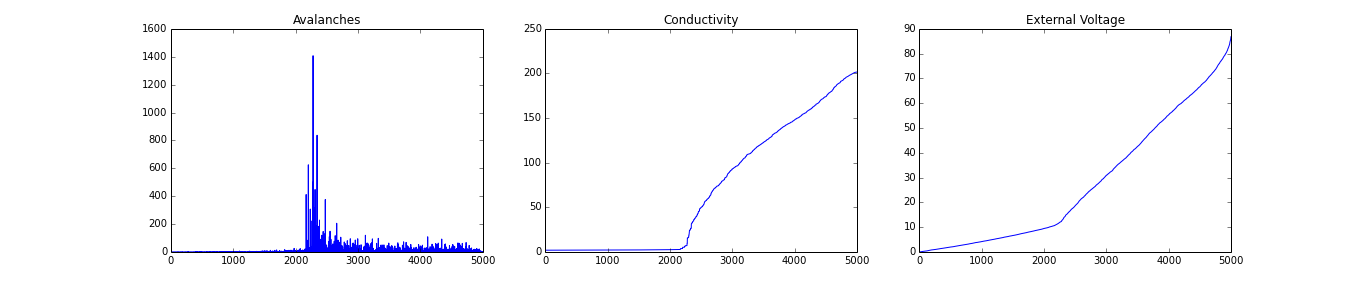
\includegraphics[width=0.8\textwidth]{ON100_run.png}
\item $g_{ON} / g_{OFF} = 1000$
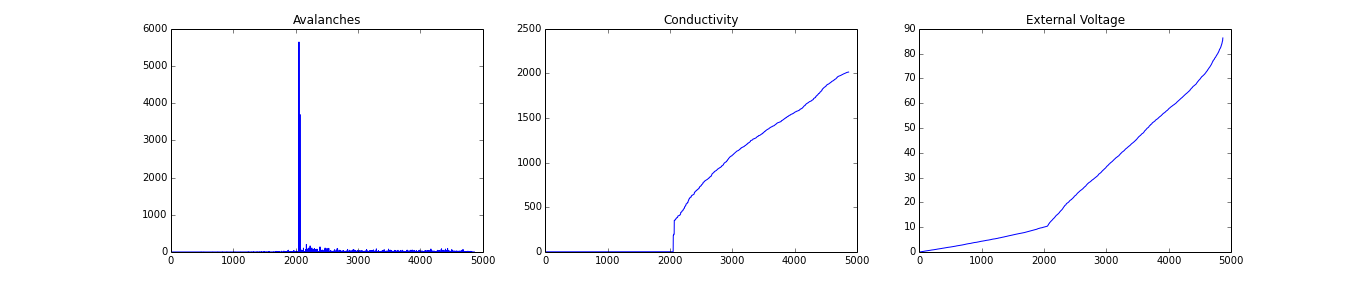
\includegraphics[width=0.8\textwidth]{ON1000_run.png}
\end{itemize}
\end{frame}

\begin{frame}
\frametitle{Internal Dynamics}
\begin{center}
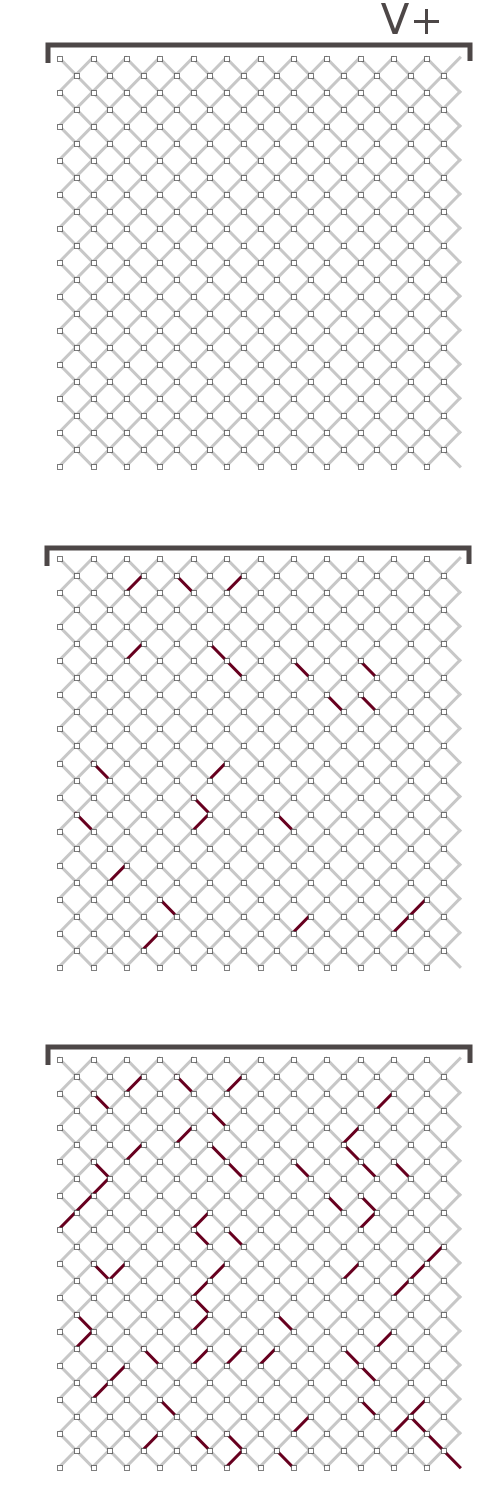
\includegraphics[width=0.8\textwidth]{Inside_a_network.png}
\end{center}
\end{frame}

\begin{frame}
\frametitle{Mean-Field Theory}
\begin{itemize}
\item Begin with $$P = \sum_i \sigma_i \Delta V_i^2$$
\item Require that the total power dissipated in the mean field model be the same
as that dissipated in the network,
$$P = G(\{\sigma_i\})V^2$$
\item Use effective medium theory to write $G(\{\sigma_i\})\approx G(\phi)$ for $\phi = \frac{\sum_i \sigma_i}{N}$
\item Insert a $\phi$ to get it back to it's original form,
$$P = \sum_i \sigma_i \frac{G(\phi)V^2}{\phi N}$$
\end{itemize}

\end{frame}

\begin{frame}
\frametitle{Mean-Field Theory}
\begin{itemize}
\item Our mean field voltage is thus
$\Delta V_{MF} = \sqrt{\frac{G(f)}{\phi(f)}}\frac{V}{\sqrt{N}}$
where I've traded $\phi$ for $f = \frac{n_{ON}}{N}$
\item From this we form a self-consistency requirement: the fraction of memristors
that have switched to $G_{ON}$ must be the fraction whose threshold is below the MF
current $g_{OFF} \sqrt{\frac{G(f)}{\phi(f)}}\frac{V}{\sqrt{N}} = h(f)v$,
$$f = \int_0^{h(f)v} p(t) dt$$
\end{itemize}
\begin{center}
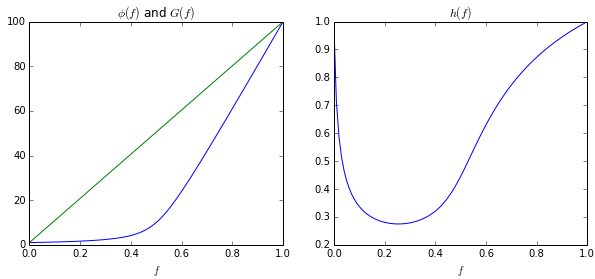
\includegraphics[width=0.6\textwidth]{MF_voltage.png}
\end{center}
\end{frame}

\begin{frame}
\frametitle{One-Dimensional Networks}
\begin{itemize}
\item In 1D, we can do this exactly!
\item For a 1D chain of conductors in series, $G(f) = \frac{g_{ON}g_{OFF}}{N(g_{ON} - f (g_{ON} - g_{OFF}))}$
$$f = \int_0^{G(f)V} p(t) dt$$
\end{itemize}
\begin{columns}
\column{0.5\textwidth}
\centering
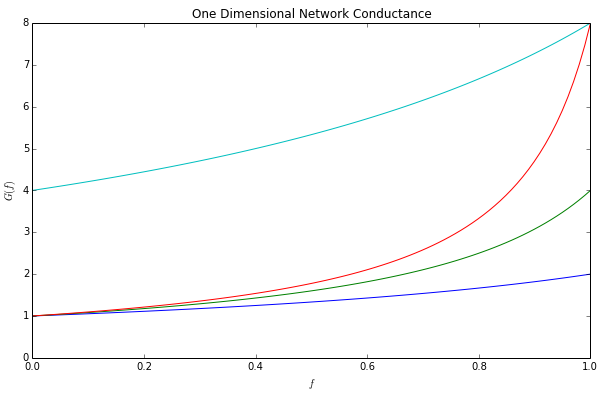
\includegraphics[width=\textwidth]{1D_Network_Cond.png}

\column{0.5\textwidth}
\centering
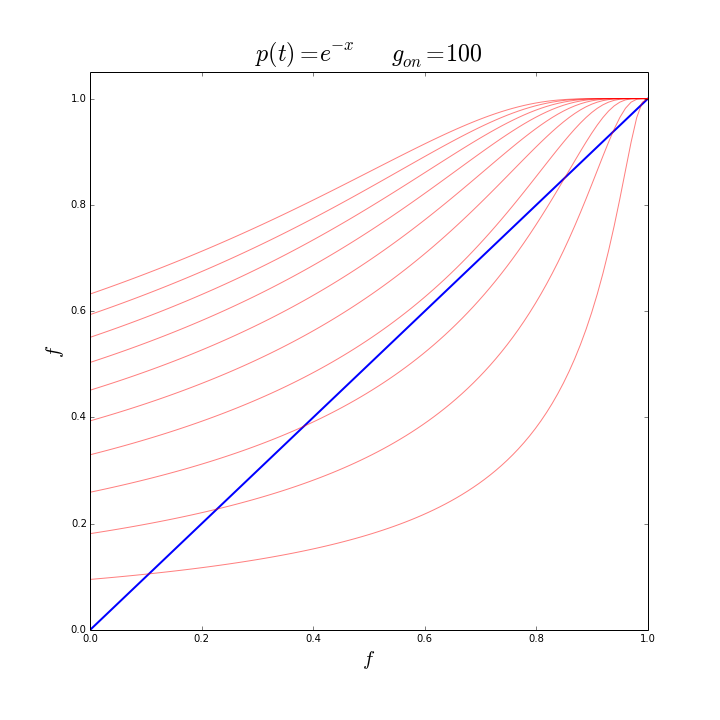
\includegraphics[width=0.9\textwidth]{SC_1D_ON100_expon.png}

\end{columns}
\end{frame}

\begin{frame}
\frametitle{Finding the transition}
First order phase transition at the solution of:
$$f = \int_0^{G(f)V} p(t) dt,  \quad 1 = p(G(f)V)G'(f)V \quad 0 \le f \le 1$$
For Uniform(0,1) this gives, 
$f_b = \frac{1}{2(1-\alpha)}, \: V_b = \frac{TN}{4g_{OFF}(1-\alpha)},
 \: \alpha = \frac{g_{OFF}}{g_{ON}}$
\centering
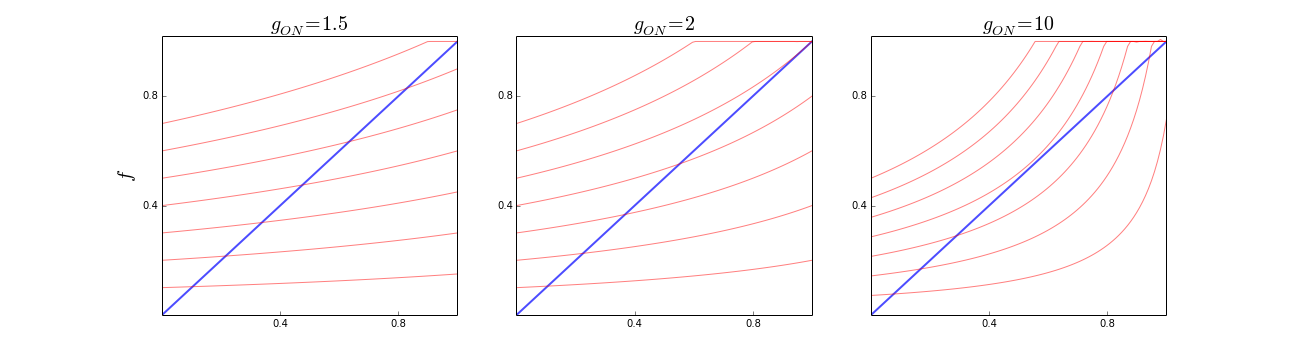
\includegraphics[width=\textwidth]{SC_1D_Uniform01.png}
\end{frame}

\begin{frame}
\frametitle{Finding the Transition}
\centering
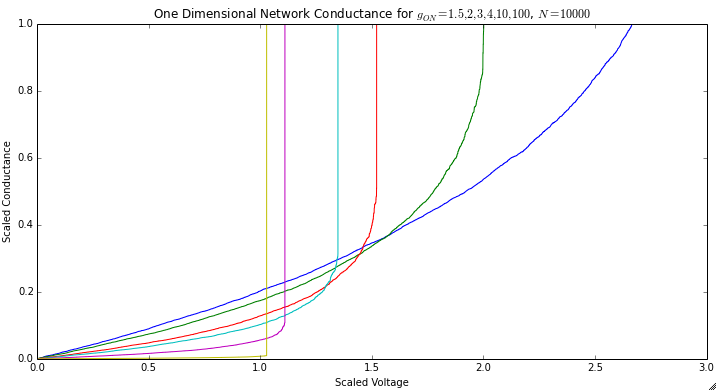
\includegraphics[width=0.8\textwidth]{1D_Cond.png}

\end{frame}

\begin{frame}
\frametitle{Back to 2D}
Inflection points from effective medium theory give us a broad transition range.
\begin{columns}
\column{0.5\textwidth}
%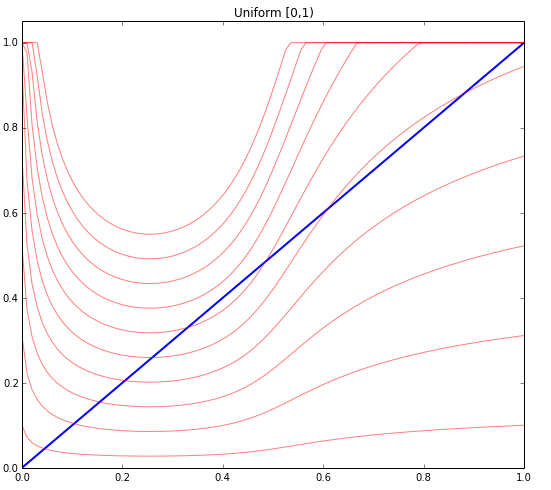
\includegraphics[width=\textwidth]{2D_MF_Uniform01.png}
\column{0.5\textwidth}
%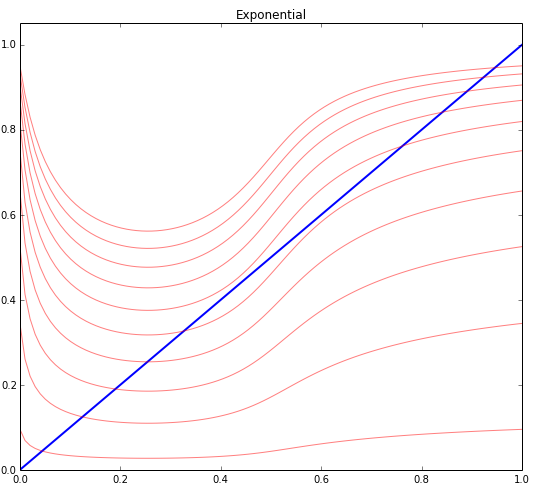
\includegraphics[width=\textwidth]{2D_MF_Exponential.png}
\end{columns}

\end{frame}

\begin{frame}
\frametitle{Avalanches}
\begin{itemize}
\item Suppose at a fraction $f$ we flip one memristor such that $f\to f'= f + \frac{1}{N}$.
\item If the MF current is an increasing function of $f$, we may have an avalanche. For large
$N$, the probability that $n$ memristors will switch in response is Poisson distributed
$$P(n) = \frac{(\mu)^n}{n!} e^{-\mu}, \quad \mu = p(h(f)v)h'(f)v$$
\item For a sequence of switchings, $S_1=1, S_2, ...,S_n, S_{n+1}=0$ the
probability distribution is
$$P(S_1, S_2, ...S_{n+1}) = \prod_i  \frac{(S_{i-1}\mu)^n}{n!} e^{-S_{i-1}\mu} $$

\end{itemize}
\end{frame}

\begin{frame}
\frametitle{Avalanche Size Distribution}
\begin{itemize}
\item Probability of observing a Poissonion branching process with total progeny $s$ is given
by the Borel Distribution,
$$P(s) = \frac{(\mu s)^{s-1}}{s!} e^{-\mu(s-1)}$$
\item As $\mu\to 1$ we approach a critical branching process and
$$P(s) \sim s^{-3/2}$$
\end{itemize}
\end{frame}

\begin{frame}
\frametitle{Avalanches in Random Resistor Networks}
%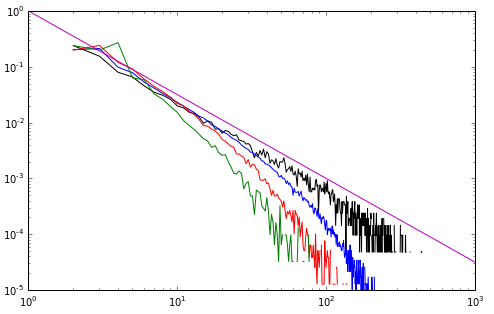
\includegraphics[width=0.8\textwidth]{Avalanches_p6.png}

\end{frame}

\begin{frame}
\begin{itemize}
\item Phase Transitions in Current Controlled Networks
\item Oscillations in Avalanches
\end{itemize}
\end{frame}

\end{document}
